\section*{Beschleunigung}
Die Beschleunigung ist eine abgeleitete Grösse. Sie gibt an, wie sich die Geschwindigkeit
mit der Zeit ändert.

Die Bewegung eines Massenpunktes heisst \emph{gradlinig gleichförmig beschleunigt}, wenn der Körper sich
mit einer konstanten Beschleunigung $a$ geradlinig bewegt.
Wird er konstant beschleunigt, ändert sich seine Geschwindigkeit linear mit der Zeit.

\begin{cbox}
\begin{gather*}
	\text{Beschleunigung} = \frac{\text{Geschwindigkeit}}{\text{Zeit}}\quad\text{oder}\quad \bar{a}=\frac{\Delta v}{\Delta t}\\
		\text{Einheit}: [a] = \frac{\text{Meter}}{\text{Sekundequadrat}}=\frac{\si{m}}{\si{s^2}}
\end{gather*}
\end{cbox}

Mit dem Strich über dem $\bar{a}$ wird angedeutet, dass eine durchschnittliche Beschleunigung 
gemeint ist.

\Einbinden{\dir/beschleunigung01.tex}
\Einbinden{\dir/beschleunigung02.tex}




\section*{Bewegungsdiagramme}
Zeitliche Bewegungsabläufe können übersichtlich in Bewegungsdiagrammen dargestellt werden.
Dabei werden die physikalischen Grössen Weg ($s$), Geschwindigkeit ($v$) und Beschleunigung ($a$) als Funktion
der Zeit dargestellt.


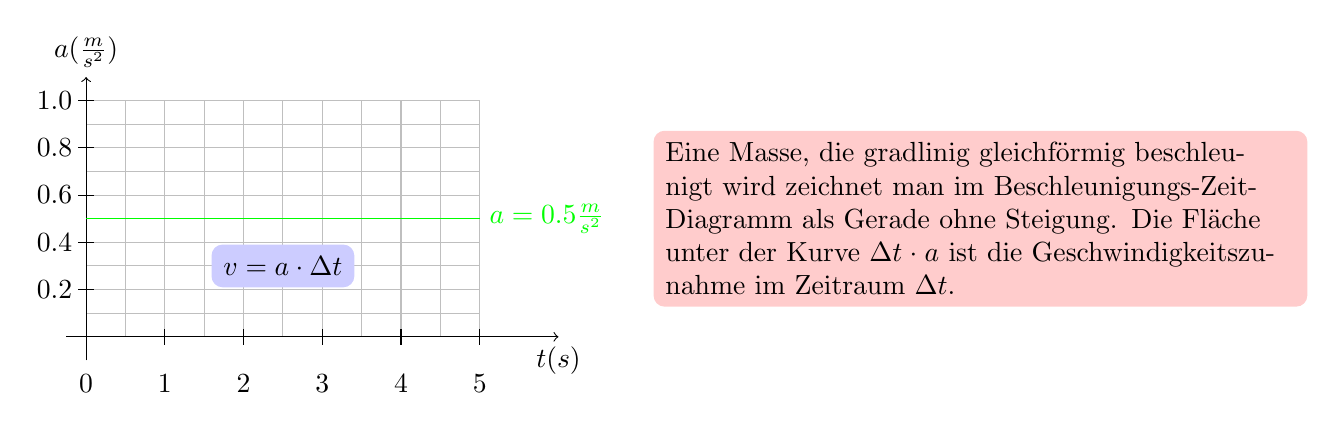
\begin{tikzpicture}[scale=1,yscale=3, info box/.style={rounded corners, inner sep=1ex}, info text/.style={info box, fill=red!20}]
\usetikzlibrary{calc,intersections,through,backgrounds}
\draw[step=0.5cm,ystep=0.1,lightgray] (0,0) grid (5.0,1.0);

%begin Koordinatensystem
%x-achse
\coordinate (C1) at (-0.25,0);
\coordinate [label=below:$t (s)$] (C2) at (6,0);
\draw  [->] (C1)--(C2);
\foreach \x in {0,1,2,3,4,5}
{
\draw (\x,-0.2) node {\x};
\draw (\x,-0.1/3)--(\x,0.1/3);
}


%y-achse
\coordinate (C3) at (0,-0.1);
\coordinate [label=above:$a (\frac{m}{s^2})$] (C4) at (0,1.1);
\draw [->] (C3)--(C4);
\foreach \y in {0.2,0.4,0.6,0.8,1.0}
{
\draw (-0.4,\y) node {\y};
\draw (-0.1,\y)--(0.1,\y);
}
%end Koordinatensystem

\draw  [color=green,domain=0:5] plot (\x,0.5) node [above,right] {$a=\SI{0.5}{\frac{m}{s^2}}$};
\draw (2.5,0.3) node [info box, fill = blue!20] {$v=a\cdot \Delta t$};

%infokasten
\draw [xshift=7.2cm] (0,0.5) node [right, text width=8cm, info text] {
Eine Masse, die  gradlinig gleichförmig beschleunigt wird zeichnet man
im Beschleunigungs-Zeit-Diagramm als Gerade ohne Steigung.
Die Fläche unter der Kurve $\Delta t\cdot a$ ist die Geschwindigkeitszunahme im Zeitraum $\Delta t$.
};



\end{tikzpicture} 


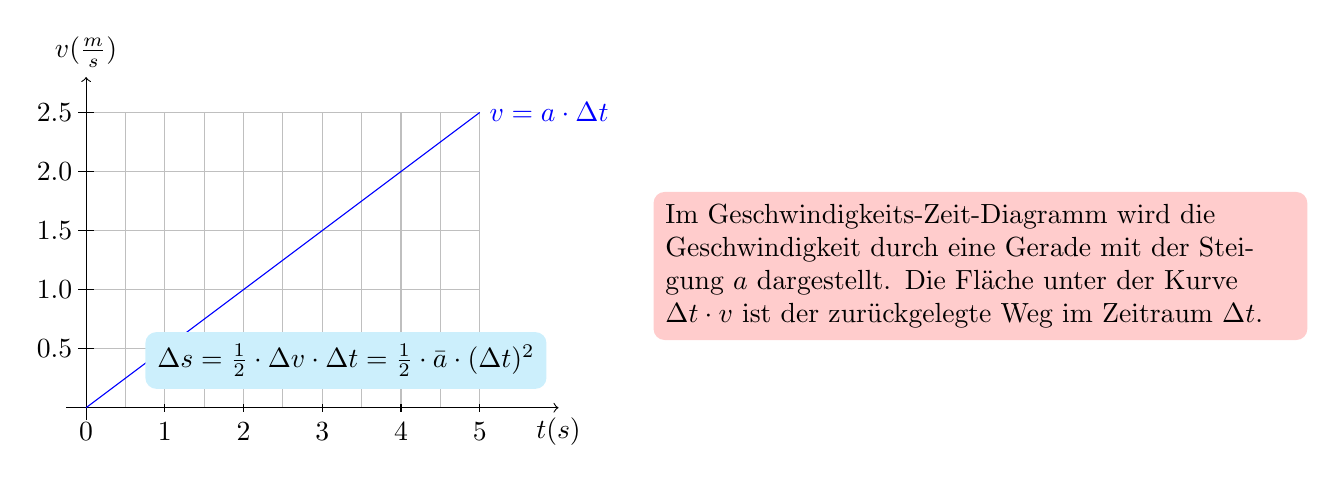
\begin{tikzpicture}[scale=1,yscale=1.5, info box/.style={rounded corners, inner sep=1ex}, info text/.style={info box, fill=red!20}]
%\usetikzlibrary{calc,intersections,through,backgrounds}
\draw[step=0.5cm,ystep=0.5,lightgray] (0,0) grid (5.0,2.5);

%begin Koordinatensystem
%x-achse
\coordinate (C1) at (-0.25,0);
\coordinate [label=below:$t (s)$] (C2) at (6,0);
\draw  [->] (C1)--(C2);
\foreach \x in {0,1,2,3,4,5}
{
\draw (\x,-0.2) node {\x};
\draw (\x,-0.1/3)--(\x,0.1/3);
}


%y-achse
\coordinate (C3) at (0,-0.1);
\coordinate [label=above:$v (\frac{m}{s})$] (C4) at (0,2.8);
\draw [->] (C3)--(C4);
\foreach \y in {0.5,1.0,1.5,2.0,2.5}
{
\draw (-0.4,\y) node {\y};
\draw (-0.1,\y)--(0.1,\y);
}
%end Koordinatensystem

\draw  [color=blue,domain=0:5] plot (\x,0.5*\x) node [above,right] {$v=a\cdot\Delta t$};
\draw (3.3,0.4) node [info box, fill =cyan!20] {$\Delta s=\frac{1}{2}\cdot \Delta v\cdot \Delta t = \frac{1}{2}\cdot\bar{a}\cdot(\Delta t)^2$};

%infokasten
\draw [xshift=7.2cm] (0,1.2) node [right, text width=8cm, info text] {
Im Geschwindigkeits-Zeit-Diagramm wird die Geschwindigkeit durch eine Gerade
mit der Steigung $a$ dargestellt. 
Die Fläche unter der Kurve $\Delta t\cdot v$ ist der zurückgelegte Weg im Zeitraum $\Delta t$.
};



\end{tikzpicture} 


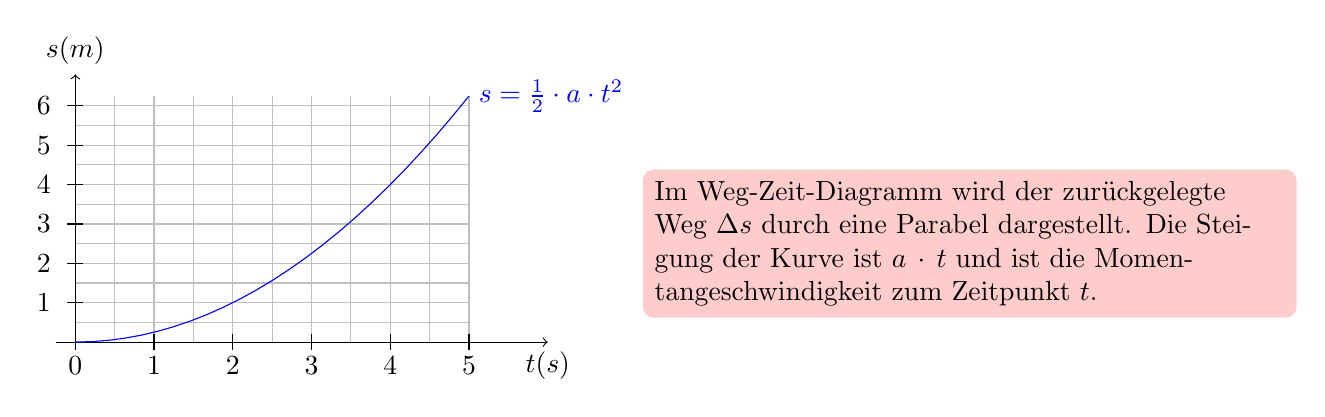
\begin{tikzpicture}[scale=1,yscale=0.5, info box/.style={rounded corners, inner sep=1ex}, info text/.style={info box, fill=red!20}]
%\usetikzlibrary{calc,intersections,through,backgrounds}
\draw[step=0.5cm,ystep=0.5,lightgray] (0,0) grid (5.0,6.25);

%begin Koordinatensystem
%x-achse
\coordinate (C1) at (-0.25,0);
\coordinate [label=below:$t (s)$] (C2) at (6,0);
\draw  [->] (C1)--(C2);
\foreach \x in {0,1,2,3,4,5}
{
\draw (\x,-0.6) node {\x};
\draw (\x,-0.1/0.5)--(\x,0.1/0.5);
}


%y-achse
\coordinate (C3) at (0,-0.1);
\coordinate [label=above:$s (m)$] (C4) at (0,6.8);
\draw [->] (C3)--(C4);
\foreach \y in {1,2,3,4,5,6}
{
\draw (-0.4,\y) node {\y};
\draw (-0.1,\y)--(0.1,\y);
}
%end Koordinatensystem

\draw  [color=blue,domain=0:5] plot (\x,0.25*\x*\x) node [above,right] {$s=\frac{1}{2}\cdot a\cdot t^2$};
%\draw (3.3,0.4) node [info box, fill =cyan!20] {$\Delta s=\frac{1}{2}\cdot \Delta v\cdot \Delta t = \frac{1}{2}\cdot\bar{a}\cdot(\Delta t)^2$};

%infokasten
\draw [xshift=7.2cm] (0,2.5) node [right, text width=8cm, info text] {
Im Weg-Zeit-Diagramm wird der zurückgelegte Weg $\Delta s$ durch eine Parabel dargestellt. 
Die Steigung der Kurve ist $a\cdot t$ und ist die Momentangeschwindigkeit zum Zeitpunkt $t$.
};



\end{tikzpicture} 




Aus den Bewegungsdiagrammen lassen sich zwei wichtige Formeln ablesen.
%\begin{cbox}
\begin{equation*}
	v=v_0+a\cdot t \qquad s=s_0 + v_0\cdot t+\frac{1}{2}\cdot a\cdot t^2
\end{equation*}
%\end{cbox}
Durch auflösen der ersten Gleichung $v=v_0+a\cdot t$ nach t und einsetzen in die zweite
bekommen wir eine Gleichung, in der die Zeit $t$ nicht vorkommt.
\begin{equation*}
	v^2=v_0^2+2\cdot a\cdot (s-s_0)
\end{equation*}

\Einbinden{\dir/beschleunigung02.tex}
